\chapter{Background and Related Work}
\label{cha:background}
The Cloud computing paradigm is shifting computing from in-house managed
hardware and software resources to virtualized Cloud-hosted
services.
Cloud computing assembles large networks of virtualized services:
infrastructure services (e.g., compute, storage, network, etc.) and software services
(e.g., databases, message queuing systems, monitoring systems, load-balancers, etc.)

Cloud providers give users the options to deploy their applications over a pool
of virtually infinite services with practically no capital
investment and with modest operating costs proportional to
the actual use. Elasticity, cost benefits and abundance of
resources motivate many organizations to migrate their
enterprise applications to the Cloud. Although the Cloud offers
the opportunity to focus on revenue growth and innovation,
decision makers (e.g., CIOs, scientists, developers,
engineers, etc.) are faced with the complexity of choosing
the right service delivery model for composite applications
and infrastructure across private, public, and hybrid Clouds.

A large number of information technology vendors claim to offer applications, storage,
and computation resources as cloud hosting services. As a
result, an exceeding number of competing services are available for
users to choose from, in such context, the migration of applications 
(e.g., multi-layered enterprise applications, scientific experiments, 
video-ondemand streaming applications, etc.) to the Cloud
demands selecting the best mix of services across multiple
layers (e.g., IaaS, PaaS, and SaaS) from an abundance of
possibilities. 
Any such Cloud service selection decision has
to cater for a number of conflicting criteria while ensuring that 
Quality of Service (QoS) requirements are met. For example, minimizing cost,
network latency, while maximizing throughput, storage space, CPU power (for analytical
programs to process more job or do it faster), RAM (bigger buffer size), etc.
QoS requirements for different applications also are varied. 
For example, scientific experiments need to meet deadlines, thus time/duration are constrained. 
On the other hand, video-on-demand streaming application need to satisfy streaming latency, resolution requirements.

Naturally, it is challenging for users to
select the right services that meet their QoS requirements in the
service cycle from selection and deployment to orchestration
(e.g., determining an optimal web service when making service
selection, identifying suitable virtual machine (VM) servers for
deploying web service instances, etc.). Effective service
recommendation techniques are becoming important to help
users (including developers) in their decision-making processes
for critical application developments and deployments. 

\section{Cloud vs. Web Service vs. Grid}

\begin{figure}[ht]
  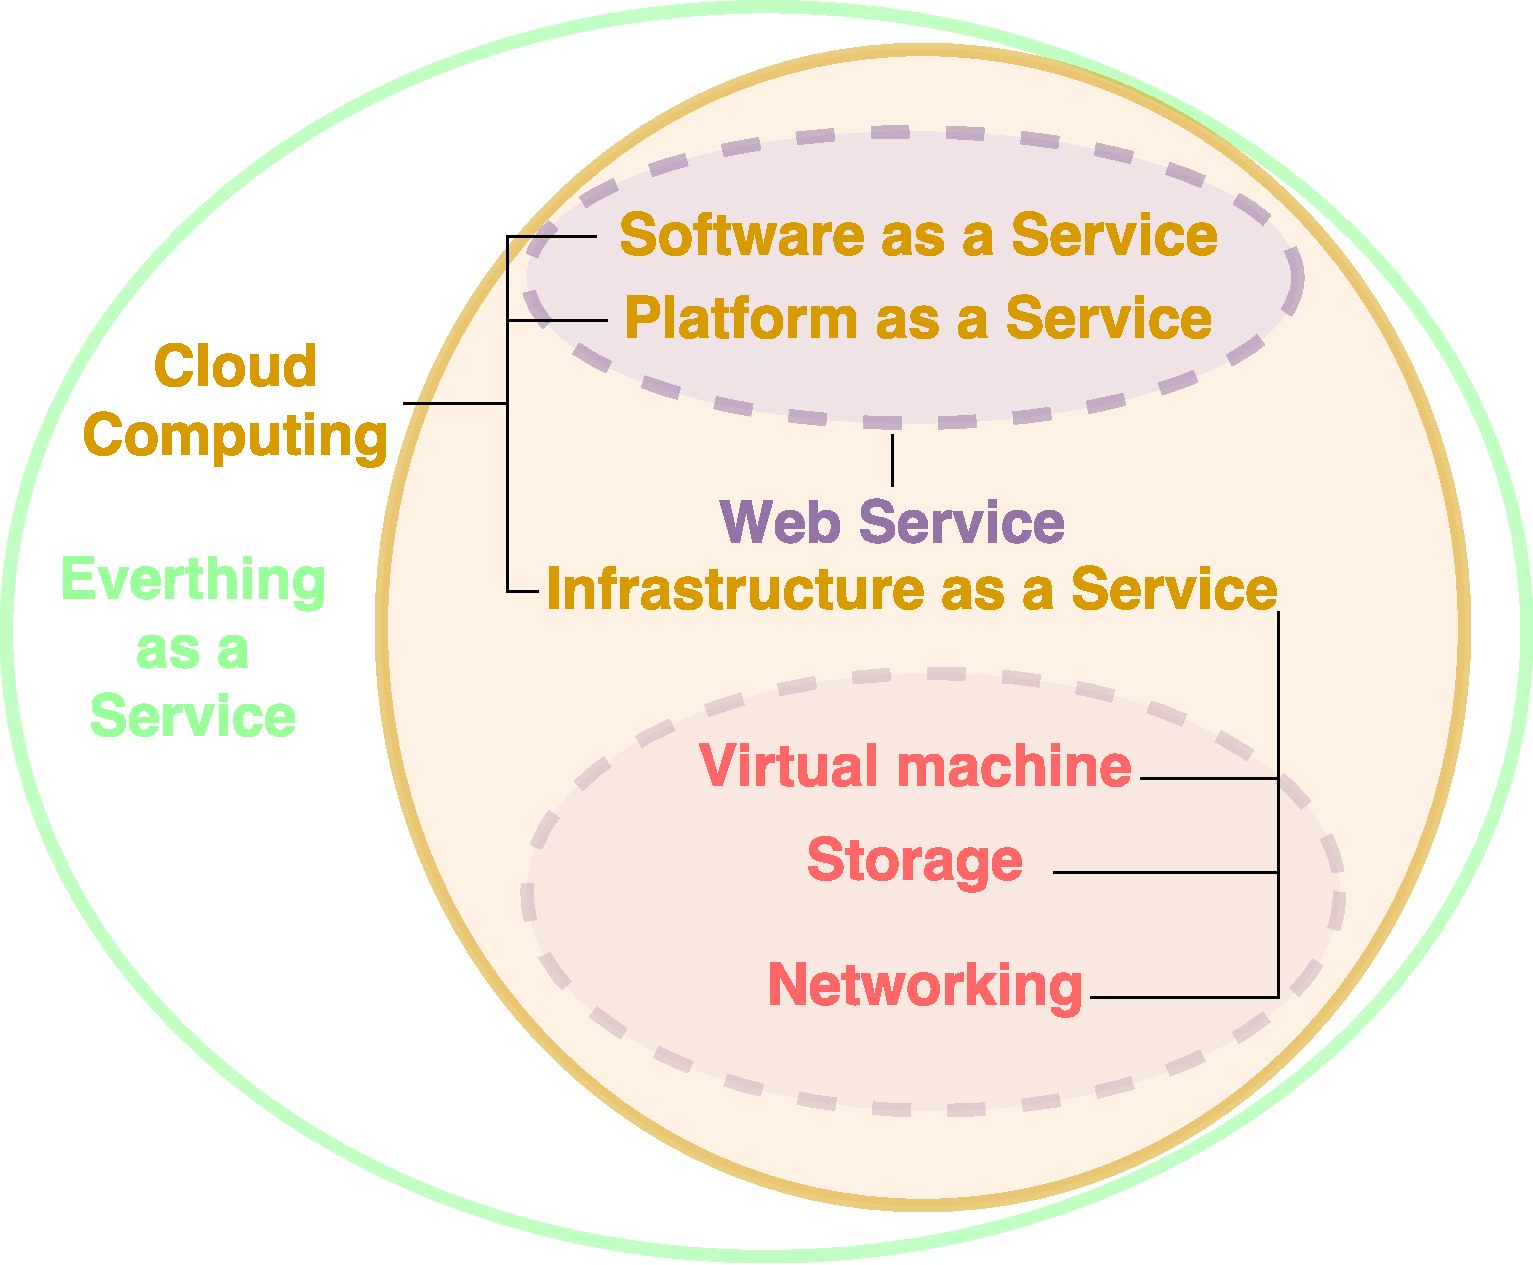
\includegraphics[width=\textwidth]{Figures/background/cloud_computing_venn.pdf}
  \caption{Cloud Computing Scope}
  \label{fig:cloud_computing}
\end{figure}
Figure \ref{fig:cloud_computing} illustrates the relationship between 
\textcolor{orange}{\textbf{Cloud Computing}}
and \textcolor{Orchid}{\textbf{Web Service}}. Web service generally does not include IaaS.

Cloud computing differs from \textbf{traditional web hosting},
mainly because of the application of \textbf{virtualization} layer.
Virtualization technology offers greater freedom resulting a
much higher scalability, and enables finer grained billing model (Pay as You Go).
see Chapter \ref{cha:system} for more information.

\textbf{Grid computing} is the collection of computer resources from multiple locations to reach a common goal. The grid can be thought of as a distributed system with non-interactive workloads that involve a large number of files \cite{grid_computing}.
In comparison, Cloud computing has more generic use cases, applicable to handle large, small or dynamic workload.

\textbf{Virtualization technique} \cite{virtualization} was developed in late 1990s and is different from simulation and emulation.
Virtualization employs techniques used to create instances of an environment, such as certain kind of virtual machine environment, note that storage and network can also be virtulized.
Full virtualization requires that every salient feature of the hardware be reflected into one of several virtual machines – including the full instruction set, input/output operations, interrupts, memory access, and whatever other elements that runs on the bare machine.

A hypervisor is computer software, firmware that creates and runs virtual machines. A computer on which a hypervisor runs one or more virtual machines is called a host machine, and each virtual machine is called a guest machine. The hypervisor presents the guest operating systems with a virtual operating platform and manages the execution of the guest operating systems. Multiple instances of a variety of operating systems may share the virtualized hardware resources: for example, Linux, Windows, and Mac OS instances can all run on a single physical x86 machine \cite{hypervisor}. See table \ref{table:hypervisor_types} for types and examples of hypervisor.

\begin{table}
    \begin{tabular}{ p{70mm} | p{70mm} }
        \hline
        \multicolumn{2}{c}{Types of Hypervisor} \\
        \hline
        Native or Bare-metal & Hosted \\
        \hline
            Run directly on the host's hardware.& 
            Run on a conventional operating system (OS)\\
        \hline
            These hypervisors run directly on the host's hardware to control the hardware and to manage guest operating systems. For this reason, they are sometimes called bare metal hypervisors.& 
            These hypervisors run on a conventional OS just as other computer programs do. A guest operating system runs as a process on the host. These hypervisors abstract guest operating systems from the host operating system.   \\
        \hline
        \multicolumn{2}{c}{Examples} \\
        \hline
            Xen \cite{xen}, Microsoft Hyper-V \cite{Hyper-V}, VMware ESX \cite{VMware_ESXi} & 
            VMware Workstation \cite{VMware_Workstation}, VMware Player, VirtualBox \cite{VirtualBox} \\
        \hline
    \end{tabular}
    \caption{Types of Hypervisors}
    \label{table:hypervisor_types}
\end{table}

\begin{figure}[ht]
  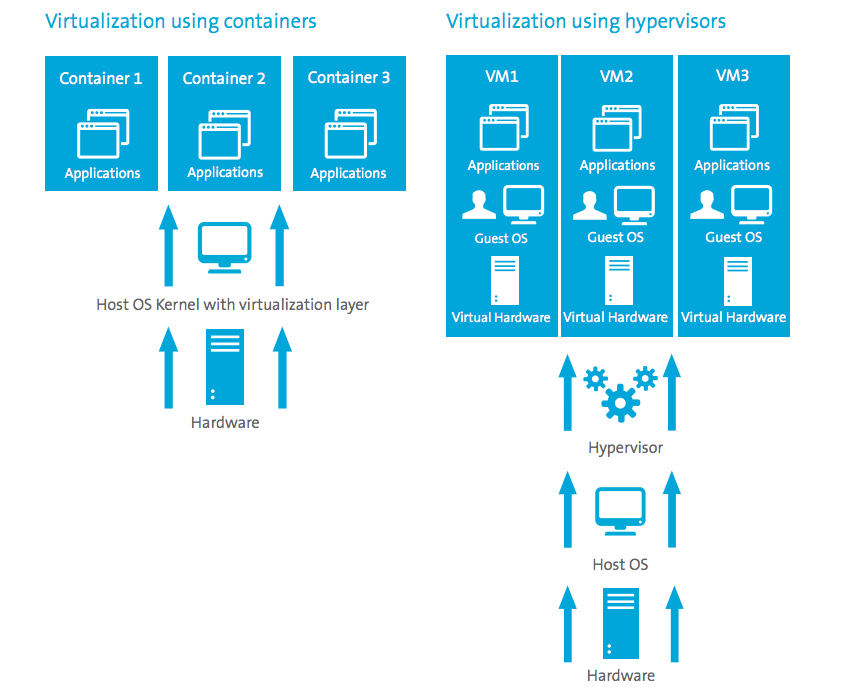
\includegraphics[width=\textwidth]{Figures/background/container_vs_hypervisor.png}
  \caption{Container vs. Hypervisor}
  \label{fig:Container_vs_Hypervisor}
\end{figure}
Operating-system-level virtualization, also known as containerization, refers to an operating system feature in which the kernel allows the existence of multiple isolated user-space instances. Such instances, called containers, may look like real computers from the point of view of programs running in them. The difference between containers and hypervisors are illustrated in \Cref{fig:Container_vs_Hypervisor}.

A computer program running on an ordinary person's computer's operating system can see all resources (connected devices, files and folders, network shares, CPU power, quantifiable hardware capabilities) of that computer. However, programs running inside a container can only see the container's contents and devices assigned to the container \cite{containerization}.
An example implementation is Docker \cite{docker}.

\textbf{Everything as a service} (EaaS, XaaS, *aaS) is initially a concept of being able to call up re-usable, fine-grained software components across a network. The most common and successful example is software as a service, but the term \enquote{as a service} has been associated and used with many core components of cloud computing including communication, infrastructure, data and platforms \cite{XaaS}.

As the term \enquote{*aaS} getting more popular, a number of vendors including Google, Microsoft, Hewlett Packard and Amazon have been associated with the "everything as a service" trend, i.e. machine learning as a service, mobile backend as a service, mechanical turk (human as a service), security and testing as a service.

XaaS is not only limited to online services. Bricks-and-mortar businesses are also being transformed through digital connectivity. Transportation-as-a-service is being fulfilled by companies like Uber and Lyft; grocery-as-a-service is being offered by chains such as Safeway and Whole Foods; and accommodation-as-a-service is a lodging rental service provided by Airbnb. This is just the tip of the iceberg with many more on their way \cite{XaaS_beyond}.

\section{Web Service Discovery Techniques}
\label{sec:WebServiceDiscoveryTechniques}
We surveyed a list of state of the art in Service Selection and Comparison techniques, we highlight their limitations, their relationship and dependency on some of the prior concepts from other fields in computing. 

Traditional \textbf{web} service discovery techniques includes Web Services Description Language (\textbf{WSDL}) and Universal Description, Discovery, and Integration (\textbf{UDDI}). UDDI has not been as widely adopted as its designers had hoped. It has been closed. On the other hand, \textbf{Semantic Web} technologies becomes popular, see \Cref{sec:semantic_web}.

Some of the "Cloud discovery" research just focused on the SaaS and PaaS domain, which I consider mostly can be categorized into web service discovery research. Other research projects may have included IaaS, but have over simplified the billing model or offering types, see section \ref{sec:research_problem} for more details about the complexity of those Cloud IaaS offers, thus impractical for most of the scenarios. I have included a summary table of related works, see \Cref{table:related_work}. Overall, projects included in this section do not include QoS into comparison. There is no reference to the code base of the implemented systems, it's impossible to reproduce results and little provide evaluation on real word data.

\begin{longtable}{ p{30mm} | p{50mm} | p{50mm} } 
\caption{Related work \label{table:related_work}} \\
\hline
\multicolumn{3}{c}{ \cellcolor{yellow} Fully Automatic Service Discovery Techniques}\\
\hline
\multicolumn{3}{p{140mm}}{All fully automatic techniques facing the same challenge of natural language processing, thus only a limited set of attributes can be captured by the proposed ontologies, and most research can only offer keyword based search, or does not consider service performance.}\\
\hline
Research Title & Proposed Method & Limitation \\ 
\hline
    A Cloud computing approach based on mobile agents for Web services discovery
    \cite{MobileAgentsWebServicesDiscovery}&
    Crawling information using mobile agents, keyword-based search is used to compare between user request and cloud service description.& 
    It does not cover numeric attributes such as cost and performance.\\
\hline
	A Crawler Engine for Cloud Services Discovery on the World Wide Web \cite{CSCE} &
    Crawl cloud web portals and store the retrieved Cloud services information in a local repository. The collected Cloud services were categorized into IaaS, PaaS and SaaS based on Ontology.&
    This research is mainly addressing the entry point problem for fully automatic discovery, the data collected from each service are limited, thus there is no mentioning of addressing the more complex need of comparing services, or filter service on certain attributes (price, VM type and RAM or performance).\\
\hline
	Design and Implementation of the Hadoop-Based Crawler for SaaS Service Discovery \cite{Hadoop-BasedCrawlerForSaaSDiscovery}.&
    Hadoop framework \cite{Hadoop} based crawler, implemented with Solr search platform \citet{ApacheSolr}.&
    Do not distinguish between IaaS, PaaS or SaaS. \\
\hline
	Integrating Software Agents and Web Services in Service Oriented Architecture Based Cloud Services Discovery Framework \cite{AgentSOAServicesDiscovery}.&
	Multi agent system for Cloud service discovery and ranking following the Service Oriented Architecture \cite{SOA}. &
    Didn't include design or method on how to implement a system follow the proposed architecture. It is critical because, tasks such as generate taxonomy tree, similarity reasoning, measure documentation and compliance, evaluate client source code, can be very complex subsystem/subproblem on its own, without a concrete ground the proposed system can not be fully realized.\\
\hline
	CSRecommender \cite{CSRecommender}&
    A search engine system called CSRecommender optimised especially for cloud services. It identifies some interested sites to crawl their web pages,
    a score is assigned to each page based on key word frequencies (i.e. TFIDF is used). It also collected users rating on the search result, to improve the recommendation relevance.&
    It was applied on few cloud services. Accuracy is low. It does not cover all types of Cloud services.\\
\hline
% Semi-automatic Service Discovery 
\multicolumn{3}{c}{\cellcolor{yellow} Semi-automatic Service Discovery with More Complex Filtering}\\
\hline
Research Title & Proposed Method & Limitation \\
\hline
    A Multi-Agent-Based QoS-Driven Web Service Discovery and Composition Framework \cite{Multi-agent-BasedCloudDescriptionDiscoveryOntology}&
    A prototype system for describing and discovering Cloud services, based on ontology and agents.&
    Requires service provider to implement agent system to interact with service registry. No evaluation with real data.\\
\hline
	Toward dynamic and attribute based publication, discovery and selection for cloud computing \cite{DynamicAttributeBasedPublicationDiscoverySelectionForCloud} &
    A schema extending WSDL, by adding attributes for describing current state of the services, e.g. Amount of free disk space or memory, Number of processes running, percent of CPU used. &
    Because of the tightly coupling with the Web Service SOAP technology stack, there is limited application on its own, SOAP is a bit out dated compare to more recent technologies. \\
\hline   
    Efficient Service Discovery for Cloud Computing Environments
    \cite{EfficientServiceDiscoveryforCloudComputingEnvironments} & 
    Store Cloud service in WSDL file for publishing in an UDDI directory.& 
    UDDI is an old (outdated) technology and abandoned by market and community.\\ 
\hline
	Cloudle \cite{Cloudle, CloudleAgent-BasedCloudComputing} & 
    Uses agents, ontology, k-means clustering algorithm to discover services over the Internet. & 
    Evaluated using virtual (provider) websites. 
    Cloud providers still need to register their services in a central database.
    Cloud ontology only covers limited attributes,
    which will affect the similarity calculated between Cloud services.\\ 
\hline
% Web service composition 
\multicolumn{3}{c}{ \cellcolor{yellow} Web Service Composition}\\
\hline
\multicolumn{3}{p{140mm}}{There are methods proposed for network-aware service composition
\cite{Yu2007, Benatallah2004, Zheng2013}
considering generic web services, i.e., at the
Software-as-a-Service and Platform-as-a-Service levels. However,
the compatibility constraints at the IaaS level are different
from those at the web service. For example, generic web
services are distinguished by their features, QoS, and prices.
It does not make sense to include two exact same services in
one composition as one job does not need to be done twice, but
using multiple quantities of an IaaS offer is perfectly valid.}\\
\hline
\end{longtable}

\section{Semantic Techniques}
\label{sec:semantic_web}
According to the W3C, "The Semantic Web provides a common framework that allows data to be shared and reused across application, enterprise, and community boundaries". The term was coined by Tim Berners-Lee for a web of data that can be processed by machines — that is, one in which much of the meaning is machine-readable. While its critics have questioned its feasibility, proponents argue that applications in industry, biology and human sciences research have already proven the validity of the original concept \cite{SemanticWeb}.

The term "Semantic Web" is often used more specifically to refer to the formats and technologies that enable it. The collection, structuring and recovery of linked data are enabled by technologies that provide a formal description of concepts, terms, and relationships within a given knowledge domain. These technologies are specified as W3C standards and some examples are:

\begin{enumerate}
    % 1
    \item 
    Resource Description Framework (RDF), a general method for describing information.
    % 2
    \item
    SPARQL, an RDF query language.
    % 3
    \item
    Web Ontology Language (OWL), a family of knowledge representation languages. For adding meaning to web content by annotating it with terms defined in ontologies.Supported by tools (e.g. Protégé) and APIs (e.g. OWL API). Based on Description Logics \cite{OntologyLanguageTool2}.
\end{enumerate}

\subsection{Ontology}
Many industries (i.e. smart factories, business analytics) are
becoming increasingly dependent on complex automatic software systems for tasks like resource allocation, business decision making, etc.
For example, to make decentralized decisions, those systems need to cooperate with each other as well as with humans.
However, those systems typically access data from different models, which have been independently developed in different (often incompatible) formats using different types of proprietary software. Furthermore, these models may not come with a well-defined semantics, and their specification can be ambiguous.
As a result, model development, maintenance, and integration, as well as data exchange and sharing pose major challenges in practice
\cite{CapturingIndustrialInformationWithOntologies}.

As a result, adoption of semantic technologies has been welcomed in many large companies such as in Google, Facebook, IBM \cite{SemanticTechnologiesInIBM}
and Siemens \cite{CapturingIndustrialInformationWithOntologies}.
For example, OWL 2 ontologies are often used to capture the conceptual information models.
OWL 2 is a rich and flexible modeling language. It not only comes with an
unambiguous, standardized, semantics, but also with a wide range of tools that can be used to
develop, validate, integrate, and reason with such models.
Data can be stored in RDF triplestores and effectively queried in conjunction with the available ontologies.
RDF is a standard model for data interchange on the Web.
RDF has features that facilitate data merging even if the underlying schemas differ,
and it specifically supports the evolution of schemas over time
without requiring all data consumers to be changed \cite{RDF}.

Like the software design patterns, many \textbf{Ontology Design patterns}(ODP) \cite{ODP}
also have been proposed to suggest standardized solutions for common problems.

\subsection{Linked Data}

In computing, linked data (often capitalized as Linked Data) is a method of publishing structured data so that it can be interlinked and become more useful through semantic queries. It builds upon standard Web technologies such as HTTP, RDF and URIs, but rather than using them to serve web pages for human readers, it extends them to share information in a way that can be read automatically by computers.

Tim Berners-Lee, director of the World Wide Web Consortium (W3C), coined the term in a 2006 design note about the Semantic Web project \cite{LinkedData}. Linked data may also be open data, in which case it is usually described as linked open data (LOD).

Some example Resource Description Framework serialization formats are RDF/XML, JSON-LD \cite{JSON-LD}. 
\subsection{Schema.org}

Schema.org \cite{Schema.org} is an initiative launched on 2 June 2011 by Bing, Google and Yahoo to "create and support a common set of schemas for structured data markup on web pages." In November 2011 Yandex (whose search engine is the largest one in Russia) joined the initiative.

The Knowledge Graph is a knowledge base used by Google and its services to enhance its search engine's results with information gathered from a variety of sources. This information is presented to users in a box to the right of search results. Knowledge Graph boxes were added to Google's search engine in May 2012. The information covered by the Knowledge Graph grew significantly after launch, tripling its original size within seven months, and being able to answer "roughly one-third" of the 100 billion monthly searches Google processed in May 2016 \cite{Knowledge_Graph}.
In October 2016, Google announced that the Knowledge Graph held over 70 billion facts. The information is often used as a spoken answer in Google Assistant and Google Home searches. 

The Knowledge Graph Search API uses standard schema.org types and is compliant with the JSON-LD specification.

The Knowledge Graph has been criticized for providing answers without source attribution.

\subsection{RDF}
\label{sec:RDF}
The purpose of RDF is to provide a structure (aka framework)
for describing identified things (aka resources) \cite{RDFandOWL_SenmanticWebAffinityGroup}.
The RDF data model is based on statements to describe and feature resources, especially web resources, in the form of subject-predicate-object (resource–property–value) expressions (RDF triples) \cite{rdf-triples}.

Structured datasets can be written in RDF using a variety of other syntax notations and data serialization formats, for example, RDFa, JSON-LD, Notation3 (N3), Turtle \cite{rdfTurtle}, etc. The N3 syntax is, for example, less verbose than the RDF/XML serialization. A subset of N3 is the Terse RDF Triple Language, often referred to as Turtle. Turtle provides a syntax to describe RDF graphs in a compact textual form, which is easy to develop. It is a subset of Notation 3 (N3) and a superset of N-Triples. Turtle is popular among Semantic Web developers and considered as an easy-to-read alternative to RDF/XML. The typical file extension of Turtle files is \texttt{.ttl}. The character encoding of Turtle files should be \texttt{UTF-8}. The MIME type of Turtle is \texttt{text/turtle}. Turtle is supported by many software frameworks that can be used for querying and analyzing RDF data, such as Jena and Sesame. Turtle files consist of a sequence of directives, statements representing triples, and blank lines.

\subsection{RDFS}
As mentioned in Section \ref{sec:RDF}, RDF allows you to link resources (concepts) together so you could say that (Karthik  is a person). Think about it as directed graph, however you can't classify objects so you can't say for example that person is a subclass of human-beings.

RDFS (RDF Schema) gives you more expressive vocabulary, this means you can start making statements about classes of thing, and types of relationship. It also allows you to describe in human readable text the meaning of a relationship or a class.
It allows you to classify resources by using the class and subclass (\texttt{rdfs:class}, \texttt{rdfs:subclass}) notions. It also allows you to set restriction on the properties(relationships) using \texttt{rdfs:Domain} and texttt{rdfs:range}.
It tells you legal uses of various classes and relationships. It is also used to indicate that a class or property is a sub-type of a more general type. For example "HumanParent" is a subclass of "Person". "Loves" is a sub-class of "Knows"\cite{RDFvsOWL_SO}.

\subsection{OWL}
The purpose of OWL is to develop ontologies that are compatible with the World Wide Web \cite{RDFandOWL_SenmanticWebAffinityGroup}.
OWL it is closely related to it to RDF, however, OWL is not an extension to RDF, in the same sense that DTDs and XML Schema are not extensions to XML \cite{RDFvsOWLquora}. 
OWL is a way of adding meaning / semantic richness to RDF.  Among other things this allows automated reasoning / influencing.
OWL is a way to define types for RDF data, though OWL "typing"  differs from conventional type systems in that it has an open world  assumption. OWL is represented using RDF triples and typically expressed using RDF/XML syntax.
OWL allows you to add more restrictions. It categorises properties(relationships) into object and data properties and allows you to add restrictions on your properties.

\subsection{Ontologies Related to Cloud}
Parra-Royon and J.M. Ben\'{i}tez~\cite{DataMiningServicedefinitionInCloud} have developed two small Cloud ontologies. The set of concepts and features they cover are limited and, as a result, their examples are limited to some simple cases. For instance, the examples presented in Section \ref{sec:PriceSpecification}
cannot be modeled with their ontologies.
Since their dataset links are now inaccessible, there is no further evidence of the applicability of their model today.

K. Boukadi et al. have developed a Cloud Service Description Ontology (CSO) \cite{Boukadi2016CloudSD}, primarily for the modeling of Cloud Service brokerage. Their price model is rather simple and cannot model real world scenarios. Their model and data are also not available online anymore to be evaluated further or to be reused in other contexts.

In the mOSAIC project~\cite{Moscato2011AnAO}, researchers proposed an OWL ontology for Cloud services negotiation (i.e. between costumers and providers) and composition (i.e. by an administrator). Their ontology is different in scope to ours.

K. Joshi et al. have developed an OWL Ontology for the Lifecycle of IT Services in the
Cloud \cite{Joshi2014AutomatingCS}. This ontology models the steps involved in the
phases of discovery, negotiation, composition, and consumption of Cloud services.
The modelling of Cloud service features is very limited, and their link to an example of a storage service \cite{kjoshi_storage_ontology} is no longer accessible.

In the area of Quality of Service (QoS) modelling, some papers have proposed QoS ontologies (i.e. QoSOnt \cite{QoSOnt} and OWL-QoS \cite{OWL-QoS}).
However, they did not publish the actual specifications, and only figures/graphs were given.
In this paper, we provide formal modelling of QoS parameters, and make it readily available for generic use (see Section \ref{sec:CloudServicePerformance}).

\Cref{table:OntologiesComparison} shows an comparison of related works with ontology.
Overall, all the other models have a different scope compared to our ontology. Our focus is on modeling functions, prices and performance of Cloud infrastructure services. 
We do not consider models for orchestration \cite{Moscato2011AnAO,Joshi2014AutomatingCS} nor brokerage processes \cite{Boukadi2016CloudSD}. Nonetheless, our ontology could be extended in this regard using the models proposed in those works.
Furthermore, we have also developed tools for automatically adding semantics to information from providers' APIs. 

We have used existing ontologies whenever fits, such as the Unit of Measure Ontology (QUDT) \cite{OntologyUnitsOfMeasure} for defining price with currency values.
\Cref{fig:ExistingOntologies} shows some of the existing ontologies, the larger the size, the more it is referenced/used by other ontologies.
\begin{figure}[ht]
  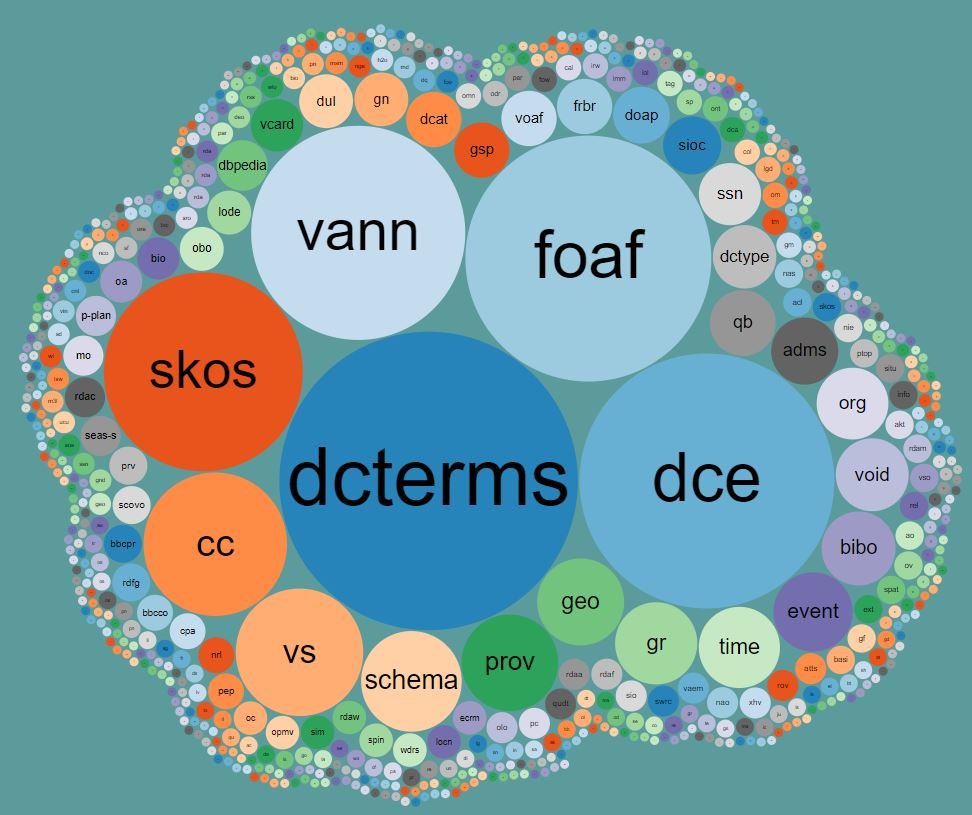
\includegraphics[width=\textwidth]{Figures/background/LOV.jpg}
  \caption{Existing Ontologies}
  \label{fig:ExistingOntologies}
\end{figure}
 For the full list of ontology we have referenced, see the online document\footnote{\url{https://github.com/miranda-zhang/cloud-computing-schema/blob/master/vocabularies.md}}.

\begin{longtable}[ht]{ p{.2\linewidth} p{.35\linewidth} p{.35\linewidth} }
\caption{Related Work using Semantic Techniques \label{table:OntologiesComparison}} \\
    \toprule
        Ontologies & Details & Limitations\\
    \midrule
    \endfirsthead
        Parra-Royon and J.M. Ben\'{i}tez~\cite{DataMiningServicedefinitionInCloud}.
        \textbf{ccsla}, \textbf{ccpricing}, \textbf{ccinstances}, \textbf{ccregions},\textbf{dmcc-schema}, \textbf{ccdm}.
        &
        Features:
            SLA, Price, VM instance feature and Region, Vendor. Data mining experiments parameters. 
       \bigskip
       
        Availability:
            Schemas and data are online. Each schema has one or two examples modelling Services from Amazon. One exception is \textbf{ccdm} which has 6 examples of different ML experiments.
        &
        \textbf{ccpricing} can not handle the complexity of most common price options, like cost of OS to be installed on the VM, network data transfer cost differed by destination and usage, snapshot storage costs and etc. See our illustrations in \ref{sec:PriceSpecification}. \textbf{ccinstances} does not allow unit to be specified in data, has to be fixed for each property.
        \\
        Cloud Service Description Ontology (CSO) \cite{Boukadi2016CloudSD}
        &
        Features:
            Cloud Price, VM instance feature and Region, Vendor.
        \bigskip
        
        Availability:
            None of the schema, data or source code is accessible.
        &
        Project resources link is no longer accessible.
        Formal ontology definition is not available, only top level topology is shown.
        Over simplified service definition, for example in the experiment "Network" is assigned a number between 0 and 100 without unit. How could this represent data transfer size and latency all together? It could be daily or yearly usage, without knowing destination, translate this to cost is impossible.
        \\
        mOSAIC project~\cite{Moscato2011AnAO}
        &
        Features:
            Actor/Consumer/Vendor, SLA, QoS, Functional/Non-Functional Property, Application Layer, Component.
        \bigskip
        
        Availability:
            The OWL file is not available, no example. One picture shows InfrastructureSoftware and Computational class, but did not show their subclasses, without the OWL file or example, we could not tell the difference between these two classes. 
        &
        This work focused on Cloud services negotiation (i.e. between costumers and providers) and composition (i.e. by an administrator). Their ontology is different in scope to our, i.e. it does not cover price.
        Only top level concepts are covered, for example there is a QoS class, but QoS is too broad, more specific classes are needed.
        \\
        OWL Ontology for the Lifecycle of IT Services in the Cloud \cite{Joshi2014AutomatingCS}
        &
        Features:
            Cloud Provider, Consumer, Auditor, Broker, SLA, Latency, Throughput, Response Time, Request for Service, Contract, Consumer Negotiation, Security Policy.
        \bigskip
        
        Availability:
            itso.owl is available online, but the link to storage\_ontology.owl is no longer accessible.
        &
        This ontology models the steps involved in the phases of discovery, negotiation, composition, and consumption of Cloud services. But the Cloud services are only defined at very top level, like IaaS, PaaS, SaaS. Although there is one example for storage service, but the schema file storage\_ontology.owl is not accessible anymore.
        \\
    \hline
        QoSOnt \cite{QoSOnt}
        &
        Features:
            Availability, Time To Complete, Throughput, Reliability, Confidentiality, Quantity, Conversion Rate.
        \bigskip
        
        Availability:
            Schema is not online, topology graphs are blurry.
        &
        This is QoS focused                                                      ontology is outdated and unavailable to use.
        \\
        OWL-QoS \cite{OWL-QoS}
        &
        Features:
            Latency, Accuracy, Reliability, Condition, Parameter, Delay and Error Tolerance.
        \bigskip
        
        Availability:
            OWL file is not available, no example.
        &
        This research proposed an QoS measurements extension to OWL-S, but the ontology isn't made available.
        \\
    \hline
    	A semantic-based Software-as-a-Service (SaaS) discovery and selection system \cite{SaaSdiscoverySelectionSystem}.
    	&
    	Features: SaaS
    	\bigskip
    	
    	Availability: OWL file is not available.
    	\bigskip
    	
    	Methods:
        Offers text/term based search. Firstly, Cloud service providers register their services, this data is  processed by consulting the WordNet \cite{WordNet} ontology to expand the service description using the token synonyms, it is  then stored in their proposed ontology. TFIDF algorithm is used to calculate weight vector for each service, then the cosine similarity between those vectors are calculated, finally the agglomerative clustering algorithm is applied to categorize services based on similarity.
        &
        Despite all the information retrieval techniques applied, it still requires service providers to register themselves manually. Ontology focused on SaaS which is different in scope. Neither of the designed ontology or data is made available, only partially shown in figures.
        \\
    	Semantic Discovery of Cloud Service Catalog Published Over Resource Description Framework \cite{Vasudevan2014SemanticDO} &
    	Features: SaaS, PaaS, SaaS
    	\bigskip
    	
    	Availability: OWL file is not available.
    	\bigskip
    	
    	Methods:
        String similarity is calculated by Levenshtein (edit) distance. Concept  similarity is calculated by finding the Least Common Hypernym (LCH) in WordNet \cite{WordNet}.The system was implemented with the Jena inference rules engine \cite{jena}.&
        Merged ontology only partially shown in figure, no experimental data is made available, making it hard to evaluate and reproduce the work.
        \\
    	Integrating intelligent agent and ontology for services discovery on cloud environment
        \cite{IntelligentAgentOntologyServicesDiscovery}
        &
        Features: PaaS
    	\bigskip
    	
    	Availability: OWL file is not available.
    	\bigskip
    	
    	Methods:
        Integrating mobile agents with ontology for searching cloud services
        using inference rules executed by Jena engine \cite{jena}.
        & 
        Despite the different method for retrieving information, the evaluation does not demonstrate much superiority compare to other researches. It achieves no more than 40 percent recall, means it can only retrieve 40 percent of what should be discovered (with human review).
        This research focus on PaaS scope, which has very different characteristic to IaaS.
        \\
    	OWL-S Based Semantic Cloud Service Broker \cite{OWL-CloudServiceBroker}
    	&
    	Features: Provider, Requester, Cost, Region, Functionality,  
    	\bigskip
    	
    	Availability: OWL file is not available, online resource no longer accessible.
    	\bigskip
    	
    	Methods:
    	Using SWRL \cite{SWRL} rule for matching criteria.
        &
        QoS parameters are not included. Only top tow levels are shown in figure, IaaS functionalities modeled are limited.
        \\
        ICT ontology \cite{Ontology-basedAnnotationRetrievalOfServicesInCloud}
        &
        Features: Software  
    	\bigskip
    	
    	Availability: OWL file is not available, \url{prefix.cc} shows the namespace \texttt{soft} is already claimed by some other ontology.
    	\bigskip
    	
    	Methods:
        Annotates cloud services descriptions in natural language using semantic techniques such as TFIDF (term frequency inverse document frequency algorithm) and ontology (OWL2).
        &
        The validation of the system was performed on a small set of services without statistical analysis on large data sets.
        Attributes covered are limited to software, features specific for Cloud are not covered.
        \\
    	Automatic Extraction of Metrics from SLAs for Cloud Service Management \cite{AutoExtractionSLA}
    	&
    	Features: SLA, Terms, Penalty, Rebate, Availability, Cost, Provider, Consumer, Location.
    	\bigskip
    	
    	Availability: OWL file is not available, prefix not defined.
    	\bigskip
    	
    	Methods:
        A prototype system, which automatically extracted the terms defined and measures of SLA documents written in text files. The extracted terms are saved as RDF graph to represent the knowledge base.
        &
        It covers SLA only. It does not provide a comparison of SLA among different providers.
        \\
    	A Cloud Repository and Discovery Framework Based on a Unified Business and Cloud Service Ontology \cite{CloudRepositoryDiscoveryFrameworkBasedonOntology}
    	&
    	Features: BusinessFunctions, Deployment Model, PaaS, Cloud Management Tools, SLA, IaaS, Server Location, Data Storage, etc.
    	\bigskip
    	
    	Availability: BusinessFunctions\_and\_Processes includes 162 subclasses. Cloud taxonomy has 157 subclasses. But OWL file is not available, prefix not defined. Classes are partially shown in figures.
        &
        Despite the large vocabulary, there is no evidence of reusing existing ontology, object properties are not shown in figures. This work has a broader coverage, while our work modeled more details for IaaS.
        \\
    \bottomrule
\end{longtable}

\section{IaaS Pricing Calculation}
Although branded calculators are available from individual cloud providers
\cite{AWSCalculator, AzurePricingCalculator, GooglePricingCalculator, RackspaceCalculator, SoftLayerCalculator}
for calculating the service leasing cost, it is not easy for users to
generalize their requirements to fit different service offers (with
various quota and limitations), let alone compute and compare
costs. 

It's hard to do decent comparison, due to the very different nature of what things are part of billing and how they are part of billing. For some, a year consists of 365 days, for others it's only 360. While it is great that Cloud vendors provide an API for pricing estimation and calculation, the very different nature of the offerings themselves make it very hard to compare them \cite{Cloudorado}.

\section{Cloud Infrastructure Service Selection Techniques}
The approaches to Cloud service selection can be categorised into:
Multiple-criteria decision-making (MCDM) based, optimization based, logic based, and others \cite{SUN2014134}.

\subsection{Multiple-criteria decision analysis}
\label{sec:MCDA}
Multiple-criteria decision analysis (MCDA) or MCDM is a sub-discipline of operations research that explicitly evaluates multiple conflicting criteria in decision making (both in daily life and in settings such as business, government and medicine). Conflicting criteria are typical in evaluating options: cost or price is usually one of the main criteria, and some measure of quality is typically another criterion, easily in conflict with the cost \cite{MCDA}.

MCDM problems are usually subdivided into continuous and discrete types. MCDM problems have two classifications: Multiple Objective Decision-making (MODM) and Multiple Attribute Decision-making (MADM). MODM methods have decision variables which are determined in a continuous or integer domain, with a large number of alternative choices. MADM methods are generally discrete, with limited number of pre-specified alternatives. Each decision matrix has four main parts, namely: (a) alternatives, (b) attributes, (c) weight or relative importance of each attribute and (d) measures of performance of alternatives with respect to the attributes\cite{MCDM}. 
Of the many MADM methods, five methods are commonly used: Simple Additive Method (SAW), Weighted Product Method(WPM), Analytical Hierarchy Process (AHP), Techniques for Order Preference by Similarity to Identical Solution (TOPSIS), a Compromise ranking method (VIKOR).

The \textbf{decision-making paradox} arises from the quest for determining reliable decision-making methods.
To find the best decision-making method a decision problem needs to be formulated, for which different decision-making methods are the alternatives. 
Since in the beginning it was assumed that the best method is not known, the problem of selecting the best method was solved by successively using different methods. The methods used in that study \cite{DecisionMakingParadox} were the weighted sum model (WSM), the weighted product model (WPM), and two variants of the analytic hierarchy process (AHP). It was found that when a method was used, say method X (which is one of the previous four methods), the conclusion was that another method was best (say, method Y). When method Y was used, then another method, say method Z, was suggested as being the best one, and so on.

The study \cite{DecisionMakingParadox} demonstrates that it is impossible to determine precisely the best decision-making method, for to do so one needs to use the best decision-making method! This problem of finding the best decision-making method always reaches a Decision-Making Paradox. However, the results of this study recommend that for most of the cases of different weights of the two evaluative criteria the revised AHP appears to be the best decision-making method of the four examined, while the original AHP, appears to be the most inaccurate one.

\subsubsection{Simple Additive Weighting (SAW) Method}
Han and Sim \cite{HanAndSim2010}, Saripalli and Pingali \cite{MADMAC}, Zhao \cite{ZHAO2012962} applied SAW in their work.
SAW method is based on the weighted average. An evaluation score is calculated for each alternative by multiplying the scaled value given to the alternative of that attribute with the weights. The weights of relative importance is directly assigned by decision maker. Followed by summing of the products for all criteria. Represented with equation would be $A_{i}=\sum w_{i}x_{ij}$,
where $A_{i}$ is the ith alternative with respect to the jth criterion.

For example, when calculating ranking with SAW, firstly,
criterion matrix with different units of measure need to be normalized,
then they are multiplied with weights.
As illustrated in Fig. \ref{fig:SAW}, suppose "Loss of life" is considered more important, i.e. given higher weight of 0.6.
"Cultural loss" has a weight of 0.1, "Economic loss" has a weight of 0.3.
After we multiply corresponding weight with each value in the standardized criterion matrix, we get the weighted criterion matrices.
Next, sum up all matrices to get one aggregated matrix.
Values are ordered from high to low, the position in the descending list is the final
ranking position, i.e. 1st is the highest value option. As shown in the figure,
the final ranking table contains the order of value from first to the tenth.

\begin{figure}[ht]
  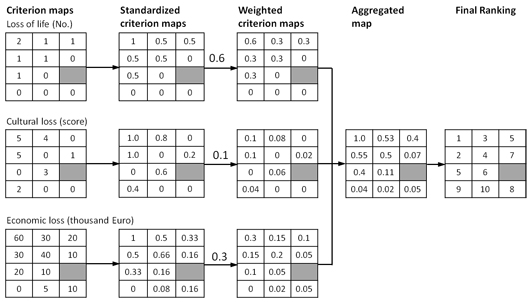
\includegraphics[width=\textwidth]{Figures/background/04_saw_method_web.jpg}
  \caption{SAW example \cite{SAWillustration}}
  \label{fig:SAW}
\end{figure}

The advantage of this method is that it is a proportional linear transformation of the raw data which means that the relative order of magnitude of the standardized scores remains equal \cite{SAW}. 

\subsubsection{Weighted Product Method (WPM)}
This method is similar to SAW.
But instead of doing addition, multiplication is used to calculated aggregated value\cite{WPM}. The normalized values are calculated as explained under the SAW method.
Suppose that a given MCDA problem is defined on m alternatives and n decision criteria. Furthermore, let us assume that all the criteria are benefit criteria, that is, the higher the values are, the better it is. Next suppose that $w_{j}$ denotes the relative weight of importance of the criterion $C_{j}$ and $a_{ij}$ is the performance value of alternative $A_{i}$ when it is evaluated in terms of criterion $C_{j}$. Then, if one wishes to compare the two alternatives $A_{K}$ and $A_{L}$ then, the following product has to be calculated:
$P(\frac{A_{K}}{A_{L}})=\prod_{j=1}^{n}(\frac{A_{Kj}}{A_{Lj}})^{w_{j}}$, for K,L=1,2,3,...,m.
If the ratio $P(\frac{A_{K}}{A_{L}})$ is greater than or equal to the value 1, then it indicates that alternative $A_{K}$ is more desirable than alternative $A_{L}$ (in the maximization case). If we are interested in determining the best alternative, then the best alternative is the one that is better than or at least equal to all other alternatives.

For example if we have the 3 alternatives each with 4 criteria as shown in
Table \ref{table:WPM_data}.
\begin{table}
\caption{Example alternatives \label{table:WPM_data}} 
\begin{center}
\begin{tabular}{ c c c c c }
\hline
&	Criteria1 &	Criteria2 &	Criteria3 &	Criteria4 \\
\hline
Weight &	0.20 &	0.15 &	0.40 &	0.25\\
\hline
Alternative1 &	25 &	20 &	15 &	30\\
Alternative2 &	10 &	30 &	20 &	30\\
Alternative3 &	30 &	10 &	30 &	10\\
\hline
\end{tabular}
\end{center}
\end{table}
WPM compare alternatives by computing a P value, like illustrated below:
$$
P(Alternative1/Alternative2)=
(\frac{25}{10})^{0.20}
*(\frac{20}{30})^{0.15}
*(\frac{15}{20})^{0.40}
*(\frac{30}{30})^{0.25}
=1.007 > 1
$$
Similarly, we also get:
$$
P(Alternative1/Alternative3)=1.067 > 1
$$
$$
P(Alternative2/Alternative3)=1.059 > 1
$$
Therefore, the best alternative is Alternative1, since it is superior to all the other alternatives. Furthermore, the following ranking of all three alternatives is as follows: A1 > A2 > A3.

It is worth noting that a useful way of choosing
between an additive score function and a multiplicative one is to consider
whether one is willing to keep giving up or trading off units of one attribute
in exchange for some units of the other attribute, at
a given fixed exchange rate, even to the point where
one has zero of the first attribute. 
If this is not acceptable to the decision maker, then the additive score
function is not appropriate.
For example, when making an investment decision, option A is more profitable, option B is safer or less risky, maximize profitability with no risk resilience left can result in disaster.
Likewise, if one does not believe the trade off rate between alternatives should stay the same however high or low, then again an additive score function is not suitable \cite{AddorMultiply}.
For example, the UNDP (United Nations Development Programme)
publishes an annual ranking of nations known as the
\href{http://hdr.undp.org}{Human Development Index},
which is very influential and is used by first world
nations to guide their aid allocations.
It is also used by pharmaceutical companies to decide which countries should receive discounted prices.
This index is an aggregate of three criteria: life expectancy, education, and gross national income per capita.
For many years the aggregation was carried out using additive weighting.
This was criticised because this assumed that the criteria were perfectly substitutable. Consequently, the UNDP chose to
change its methodology, and the index
is now calculated using a multiplicative scheme.

\subsubsection{Analytical Hierarchy Process}
One of the most popular analytical techniques for
complex decision-making problems is the analytical hierarchy process (AHP)\cite{MCDM}.
There are a number of literatures \cite{SMICloud, GodseAndMulik2009, Karim:2013:EQM:2552868.2552917, 10.1007/978-3-642-25194-8_42, nizamani2012quality} applied AHP or its variation Analytical Network Process.
AHP \cite{SAATY19909} decomposes a decision-making problem into a system of hierarchies of objectives, attributes and alternatives. An AHP hierarchy can have as many levels as needed to fully characterize a particular decision situation. A number of functional characteristics make AHP a useful methodology. These include the ability to handle decision situations involving subjective judgments, multiple decision makers and the ability to provide measures of consistency of preference.
AHP continues to be the most highly regarded and widely used decision-making method, because it is designed to reflect the way people actually think. AHP can efficiently deal with tangible as well as non-tangible attributes, especially where the subjective judgments of different individuals constitute an important part of the decision process.

\begin{figure}[ht]
  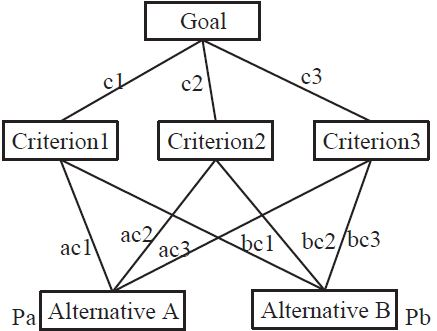
\includegraphics[width=\textwidth]{Figures/background/AHP.jpg}
  \caption{AHP \cite{SUN2014134}}
  \label{fig:AHP}
\end{figure}

\Cref{fig:AHP} shows a typical AHP hierarchy, which aims to evaluate the alternatives A and B in terms of criterion1, criterion2 and criterion3 under the overall goal.
The second phase is the comparative judgment phase.
Pair-wise comparisons are applied to determine how elements at one level influence an element at a higher level.
In \Cref{fig:AHP}, c1,c2, and c3 represent the priorities of criterion1, criterion2, and criterion3 with respect to the goal.The values of aci and bci (i=1,2,3) indicate the influence of the alternatives with respect to the criteria. In the third phase, the priorities of the elements are synthesized to induce the priorities of alternative A and B, which is achieved by:
$$
\begin{bmatrix}
c1 & c2 & c3
\end{bmatrix}
\cdot
\begin{bmatrix}
ac1 & bc1 \\
ac2 & bc2 \\
ac3 & bc3
\end{bmatrix}
=
\begin{bmatrix}
Pa & Pb
\end{bmatrix}
$$

Belton and Gear \cite{revisedAHP} propose \textbf{a revised version of the AHP model}. They demonstrate that an inconsistency can occur when the AHP is used. A numerical example is presented that consists of three criteria and three alternatives, i.e. A1, A2, A3.
The indication of the best alternative changes when an identical non-optimal alternative is introduced. For example, original ranking is A1 > A2 > A3, but after introducing another A3, the rank changed maybe to A2 > A1 > A3, A3
According to the authors, the root for that inconsistency is the fact that the relative values for each criterion sum up to one. Instead of having the relative values of the alternatives sum up to one, they propose to divide each relative value by the maximum value of the relative values.

For example, the original step normalise eigenvector into:
$$\begin{bmatrix}
\frac{1}{11} \\
\frac{9}{11} \\
\frac{1}{11}
\end{bmatrix}$$

The revised method would normalise those to:
$$\begin{bmatrix}
\frac{1}{9} \\
1 \\
\frac{1}{9}
\end{bmatrix}$$

\subsubsection{Technique for Order Preference by Similarity to Identical Solution (TOPSIS)}
This method is based on the concepts that the chosen alternative should have the shortest Euclidean distance to ideal solution and the farthest from negative ideal solution \cite{MCDM}. The ideal solution is a hypothetical solution for which all attribute values corresponds to the maximum attribute values comprising the satisfying solutions; the negative ideal solution is the hypothetical solution for which all attribute values corresponds to the minimum attribute values.
For example, if the alternatives are: [1,3], [4,2], [5,2], then the ideal solution would be [5,3], the negative ideal solution would be [1,2].
TOPSIS thus gives a solution that is not only closest to the hypothetically best, that is also the farthest from hypothetically worst.

TOPSIS can suffer from ranking abnormality \cite{SAWvsTOPSIS}.
Ranking abnormality means that the ranking of candidate networks changes when low ranking alternative is removed from the candidate list.

\subsubsection{Compromise Ranking method (VIKOR)}
The VIKOR method determines a compromise solution, providing a maximum "group utility" for the majority and a minimum of an "individual regret" for the "opponent" \cite{VIKORformula}.

The MCDM problem is stated as follows: Determine the best (compromise) solution in a multi-criteria sense from the set of J feasible alternatives $A_{1}, A_{2}$ \textellipsis $A_{J}$, evaluated according to the set of n criterion functions. The input data are the elements $f_{ij}$ of the performance (decision) matrix, where $f_{ij}$ is the value of the i-th criterion function for the alternative $A_{j}$.

The VIKOR procedure has the following steps \cite{VIKOR_method_wiki}:
\begin{enumerate}
    \item Determine the best $f_{i}^{*}$ and the worst $f_{i}^{-}$ values of all criterion functions, i = 1,2,...,n; if the i-th function is benefit:
    $$f_{i}^{*} =  \max\limits_{j} f_{ij} , f_{i}^{-} = \min\limits_{j} f_{ij}$$
    If the i-th function is cost:
    $$f_{i}^{*} = \min\limits_{j} f_{ij} ,f_{i}^{-} = \max\limits_{j} f_{ij}$$
    \item Compute the values $S_{j}$ and $R_{j}$, where j=1,2,...,J, by the relations: 
    
    Weighted and normalized Manhattan distance:
    $$S_{j}=\sum_{i=1}^{n} w_{i} \frac{f_{i}^{*} - f_{ij}}{f_{i}^{*} - f_{i}^{-}}$$
    Weighted and normalized Chebyshev distance:
    $$R_{j}=\max\limits_{i} w_{i} \frac{f_{i}^{*} - f_{ij}}{f_{i}^{*} - f_{i}^{-}}$$
    where $w_{i}$ are the weights of criteria, expressing their relative importance.
    \item Compute the values $Q_{j}$, where j=1,2,…,J, by the relation
    $$Q_{j} = v \frac{S_{j}-S^{*}}{S^{-}-S^{*}} + (1-v)\frac{R_{j}-R^{*}}{R^{-}-R^{*}}$$
    where 
    $$ S^{*} = \min\limits_{j} S_{j},
    S^{-} = \max\limits_{j} S_{j} $$
    $$ R^{*} = \min\limits_{j} R_{j},
    R^{-} = \max\limits_{j} R_{j} $$
    and v is introduced as a weight for the strategy of maximum group utility, whereas 1-v is the weight of the individual regret.
    \item Rank the alternatives, sorting by the values S, R and Q, from the minimum value. The results are three ranking lists.
    \item Propose A(1) as a compromise solution which is the best ranked by the measure Q (minimum) if the following two conditions are satisfied:
    \begin{enumerate}
        \item C1: “Acceptable Advantage”: $Q(A_{2})-Q(A_{1}) >= DQ$
        where: $A_{2}$ is the alternative with the second position in the ranking list by Q; $DQ = \frac{1}{J-1}$, J is the number of alternatives.
        \item C2: “Acceptable Stability in decision making”: The alternative $A_{1}$ must also be the best ranked by S or/and R. This compromise solution is stable within a decision making process, which could be the strategy of maximum group utility (when v > 0.5 is needed), or “by consensus” v about 0.5, or “with veto” v < 0.5).
    \end{enumerate}
    If one of the conditions is not satisfied, then a set of compromise solutions is proposed, which consists of:
    \begin{enumerate}
        \item Alternatives $A_{1}$ and $A_{2}$ if only the condition C2 is not satisfied, or
        \item Alternatives $A_{1},A_{2}$,...,$A_{M}$ if the condition C1 is not satisfied; $A_{M}$ is determined by the relation $Q(A_{M})-Q(A_{1}) < DQ$ for maximum M (the positions of these alternatives are “in closeness”).
    \end{enumerate}
\end{enumerate}

The obtained compromise solution could be accepted by the decision makers because it provides a maximum utility of the majority (represented by min S), and a minimum individual regret of the opponent (represented by min R).

\subsubsection{Preference Ranking Organization Method for Enrichment Evaluation}
The \textbf{P}reference \textbf{R}anking \textbf{O}rganization \textbf{METH}od for \textbf{E}nrichment of \textbf{E}valuations (PROMETHEE) and its descriptive complement geometrical analysis for interactive aid are better known as the Promethee and Gaia methods \cite{Promethee}.
The descriptive approach, named Gaia, allows the decision maker to visualize the main features of a decision problem: he/she is able to easily identify conflicts or synergies between criteria, to identify clusters of actions and to highlight remarkable performances.
The prescriptive approach, named Promethee, provides the decision maker with both complete and partial rankings of the actions \cite{PROMETHEE_MLwiki}.

While it can be used by individuals working on straightforward decisions, the Promethee Gaia method is most useful where groups of people are working on complex problems, especially those with several multi-criteria, involving a lot of human perceptions and judgments, whose decisions have a long-term impact. It has unique advantages when important elements of the decision are difficult to quantify or compare, or where collaboration among departments or team members are constrained by their different specializations or perspectives.

\subsection{Other Research Work}
Swinburne University has a research project called 
Smart Cloud Broker Service \cite{OpenMarketforTradingCloudServices}.
From the screen-cast they released, we can tell that their
benchmarking is done in real time, which means that users
have to wait for the results to come back. We have considered
this kind of situation but decided to collect the benchmarking
result beforehand. This is because this way, no matter how
many cloud providers users want to compare against, they can
still get the result with minimum (or no) waiting time. Another
reason we choose to do it this way is because, at any particular
point in time, the network benchmark result is not conclusive as
performance fluctuates during time; thus, we use an aggregated
average, which is a more reliable overall indication.

Menzel and Ranjan introduced a framework called
“CloudGenius” \cite{CloudGenius} that supports a decision-making process on web
server migration into the cloud. Our system supplements and
partially extends their work. CloudGenius \cite{CloudGenius} focuses on
VM selection, which means that it considers the software requirements
(i.e., the operating system version and the supported
languages), but our study focuses more on the hardware requirements
(i.e., the size of memory and hard disk). Although we
have borrowed the idea of using the AHP (with modification) from CloudGenius,
we used it differently. We have implement the method while following the declarative programming
paradigm, which should be easier to scale out as opposed to rewriting an imperative code implementation.

There are methods proposed for network-aware service composition
\cite{Yu2007, Benatallah2004, Zheng2013}
considering a generic web service, i.e., at the
Software-as-a-Service and Platform-as-a-Service levels. However,
the compatibility constraints at the IaaS level are different
from those at the web service. For example, generic web
services are distinguished by their features, QoS, and prices.
It does not make sense to include two exact same services in
one composition as one job does not need to be done twice, but
using multiple quantities of an IaaS offer is perfectly valid.
